\documentclass{beamer}
\usepackage[utf8]{inputenc}

\usetheme{Madrid}
\usecolortheme{default}
\usepackage{amsmath,amssymb,amsfonts,amsthm}
\usepackage{txfonts}
\usepackage{tkz-euclide}
\usepackage{listings}
\usepackage{adjustbox}
\usepackage{array}
\usepackage{tabularx}
\usepackage{gvv}
\usepackage{lmodern}
\usepackage{circuitikz}
\usepackage{tikz}
\usepackage{graphicx}

\setbeamertemplate{page number in head/foot}[totalframenumber]

\usepackage{tcolorbox}
\tcbuselibrary{minted,breakable,xparse,skins}



\definecolor{bg}{gray}{0.95}
\DeclareTCBListing{mintedbox}{O{}m!O{}}{%
  breakable=true,
  listing engine=minted,
  listing only,
  minted language=#2,
  minted style=default,
  minted options={%
    linenos,
    gobble=0,
    breaklines=true,
    breakafter=,,
    fontsize=\small,
    numbersep=8pt,
    #1},
  boxsep=0pt,
  left skip=0pt,
  right skip=0pt,
  left=25pt,
  right=0pt,
  top=3pt,
  bottom=3pt,
  arc=5pt,
  leftrule=0pt,
  rightrule=0pt,
  bottomrule=2pt,
  toprule=2pt,
  colback=bg,
  colframe=orange!70,
  enhanced,
  overlay={%
    \begin{tcbclipinterior}
    \fill[orange!20!white] (frame.south west) rectangle ([xshift=20pt]frame.north west);
    \end{tcbclipinterior}},
  #3,
}
\lstset{
    language=C,
    basicstyle=\ttfamily\small,
    keywordstyle=\color{blue},
    stringstyle=\color{orange},
    commentstyle=\color{green!60!black},
    numbers=left,
    numberstyle=\tiny\color{gray},
    breaklines=true,
    showstringspaces=false,
}
%------------------------------------------------------------
%This block of code defines the information to appear in the
%Title page
\title %optional
{2.8.31}
\date{September 6,2025}
%\subtitle{A short story}

\author % (optional)
{Sai Hasini Pappula-EE25BTECH11044}
\begin{document}

% --- Frame 1: Question ---
\begin{frame}{Question}
\begin{block}{Problem}
Given points $A(1,-2)$, $B(2,3)$, $C(a,2)$ and $D(-4,-3)$ which form a parallelogram. 

\begin{itemize}
    \item Find the value of $a$.
    \item Find the height of the parallelogram taking $AB$ as base.
\end{itemize}
\end{block}
\end{frame}

% --- Frame 2: Step 1 ---
\begin{frame}{Step 1: Represent the Vectors}
Represent the points as vectors:
\begin{equation}
\vec A=\begin{pmatrix}1\\-2\end{pmatrix},\quad 
\vec B=\begin{pmatrix}2\\3\end{pmatrix},\quad 
\vec C=\begin{pmatrix}a\\2\end{pmatrix},\quad 
\vec D=\begin{pmatrix}-4\\-3\end{pmatrix}.
\end{equation}

Condition for parallelogram (diagonals bisect):
\begin{equation}
\vec A+\vec C=\vec B+\vec D.
\end{equation}
\end{frame}

% --- Frame 3: Step 2 ---
\begin{frame}{Step 2: Solve for $a$}
Substituting:
\begin{equation}
\begin{pmatrix}1\\-2\end{pmatrix}+\begin{pmatrix}a\\2\end{pmatrix}
=\begin{pmatrix}2\\3\end{pmatrix}+\begin{pmatrix}-4\\-3\end{pmatrix}.
\end{equation}

Simplify RHS:
\begin{equation}
\begin{pmatrix}2\\3\end{pmatrix}+\begin{pmatrix}-4\\-3\end{pmatrix}
=\begin{pmatrix}-2\\0\end{pmatrix}.
\end{equation}

Thus:
\begin{equation}
\begin{pmatrix}1+a\\0\end{pmatrix}=\begin{pmatrix}-2\\0\end{pmatrix}.
\end{equation}

So,
\begin{equation}
1+a=-2 \;\;\Longrightarrow\;\; a=-3.
\end{equation}

Hence,
\begin{equation}
\vec C=\begin{pmatrix}-3\\2\end{pmatrix}.
\end{equation}
\end{frame}

% --- Frame 4: Step 3 ---
\begin{frame}{Step 3: Base and Side Vectors}
Base vector:
\begin{equation}
\vec B-\vec A=\begin{pmatrix}1\\5\end{pmatrix}.
\end{equation}

Side vector:
\begin{equation}
\vec D-\vec A=\begin{pmatrix}-5\\-1\end{pmatrix}.
\end{equation}
\end{frame}

% --- Frame 5: Step 4 ---
\begin{frame}
{Step 4: \[
\text{The projection of }\vec{D}-\vec{A}\text{ on }\vec{B}-\vec{A} 
\]}
\[
\text{The projection of }\vec{D}-\vec{A}\text{ on }\vec{B}-\vec{A}\text{ is } 
\]
\begin{equation}
\mathbf{P-A = \frac{(B-A)^\top (D-A)}{\|B-A\|^2} (B-A)}
\end{equation}

Compute inner products:
\begin{equation}
(\vec B-\vec A)^\top(\vec D-\vec A)=1(-5)+5(-1)=-10
\end{equation}
\begin{equation}
\|\vec B-\vec A\|^2=1^2+5^2=26.
\end{equation}

So,
\begin{equation}
\vec P-\vec A
=\frac{-10}{26}\begin{pmatrix}1\\5\end{pmatrix}
=\begin{pmatrix}-\tfrac{5}{13}\\[4pt]-\tfrac{25}{13}\end{pmatrix}.
\end{equation}
\end{frame}

% --- Frame 6: Step 5 ---
\begin{frame}{Step 5: Perpendicular Component}
Perpendicular component:
\begin{equation}
\vec r=(\vec D-\vec A)-(\vec P-\vec A)
=\begin{pmatrix}-5\\-1\end{pmatrix}
-\begin{pmatrix}-\tfrac{5}{13}\\[4pt]-\tfrac{25}{13}\end{pmatrix}
=\begin{pmatrix}-\tfrac{60}{13}\\[4pt]\tfrac{12}{13}\end{pmatrix}.
\end{equation}

Height:
\begin{equation}
h=\|\vec r\|
=\sqrt{\left(-\tfrac{60}{13}\right)^2+\left(\tfrac{12}{13}\right)^2}.
\end{equation}
\end{frame}

% --- Frame 7: Final Answer ---
\begin{frame}{Final Answer}
\[
h=\frac{\sqrt{3744}}{13}
=\frac{12\sqrt{26}}{13}
=\frac{24}{\sqrt{26}}
\]

\[
\boxed{a=-3},\qquad \boxed{h=\tfrac{12\sqrt{26}}{13}}
\]
\end{frame}
% --- Frame: C Code (Part 1) ---
\begin{frame}[fragile]{C Code (1/2)}
\begin{lstlisting}[language=C]
#include <stdio.h>
#include <math.h>

double norm(double v[2]) {
    return sqrt(v[0]*v[0] + v[1]*v[1]);
}

int main() {
    double A[2] = {1, -2};
    double B[2] = {2, 3};
    double D[2] = {-4, -3};
    double C[2];
    
    // Find 'a' using parallelogram condition: A + C = B + D
    C[0] = (B[0] + D[0]) - A[0];
    C[1] = 2;   // given y-coordinate
    printf("a = %lf\n", C[0]);
\end{lstlisting}
\end{frame}

% --- Frame: C Code (Part 2) ---
\begin{frame}[fragile]{C Code (2/2)}
\begin{lstlisting}[language=C]
    // Vectors
    double u[2] = {B[0]-A[0], B[1]-A[1]};
    double v[2] = {C[0]-A[0], C[1]-A[1]};
    
    // Projection of v on u
    double dot_uv = u[0]*v[0] + u[1]*v[1];
    double dot_uu = u[0]*u[0] + u[1]*u[1];
    double proj[2] = { (dot_uv/dot_uu)*u[0], (dot_uv/dot_uu)*u[1] };
    
    // Perpendicular component
    double w[2] = { v[0]-proj[0], v[1]-proj[1] };
    double h = norm(w);
    
    printf("Height = %lf\n", h);
    return 0;
}
\end{lstlisting}
\end{frame}

    


% --- Frame 7: Python code (1/1) ---
\begin{frame}[fragile]{Python Code (1/2)}
\begin{lstlisting}[language=Python]
import numpy as np
import matplotlib.pyplot as plt

def norm(v):
    return np.sqrt(np.dot(v, v))

# Points
A = np.array([1, -2], dtype=float)
B = np.array([2,  3], dtype=float)
C = np.array([None, 2], dtype=float)
D = np.array([-4, -3], dtype=float)

# Find a using parallelogram condition
a_val = (B[0] + D[0]) - A[0]
C[0] = a_val
print("a =", a_val)
\end{lstlisting}
\end{frame}

% --- Frame 8: Python code (part 2) ---
\begin{frame}[fragile]{Python Code (2/2)}
\begin{lstlisting}[language=Python]
# Base and AC vectors
u = B - A
v = C - A

# Projection
proj = (np.dot(v,u)/np.dot(u,u)) * u
w = v - proj
h = norm(w)
print("Height =", h)

# Plot
fig, ax = plt.subplots()
x_vals = [A[0],B[0],C[0],D[0],A[0]]
y_vals = [A[1],B[1],C[1],D[1],A[1]]
ax.plot(x_vals, y_vals, 'k-')
ax.plot([C[0], (A+proj)[0]], [C[1], (A+proj)[1]], 'r-')
plt.show()
\end{lstlisting}
\end{frame}

% --- Frame 9: Plot ---
\begin{frame}{Parallelogram Plot}
\begin{center}
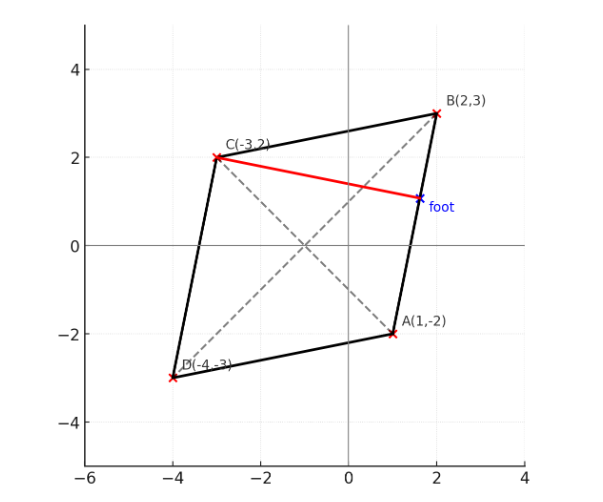
\includegraphics[width=0.7\columnwidth]{figs/fig4.png}
\end{center}
\end{frame}

\end{document}